\section{Suspendable actors}

In addition to our work, we also want to resolve a small problem that is: how to \textit{pause} an actor? And what does \textit{paused} means for an actor?

\textcolor{ForestGreen}{\textbf{When an actor receives a \textit{pause} command in a certain $S_x$ state, from this moment it will not handle any messages until he receives the \textit{resume} command, then it regularly returns to $S_x$ state at the same conditions it was before pausing}}.

So, what appends to the messages that are received while the actor is paused? There are two possibilities:
\begin{enumerate}
	\item the messages are \textbf{ignored} and discarded;
	\item the messages are \textbf{restored} and handled by the actor when it receives the \texttt{resume} command.
\end{enumerate}

Obviously, the \texttt{pause} and \texttt{resume} command are \textbf{messages} with a dedicated and fixed id. We choose to use \texttt{sys\_suspend\_actor} and \texttt{sys\_resume\_actor} as the ids for \texttt{pause} and \texttt{resume}.
We also decide to let the application designer to choose how to manage the messages while an actor is in pause.

\begin{figure}[h!]
	\centering
	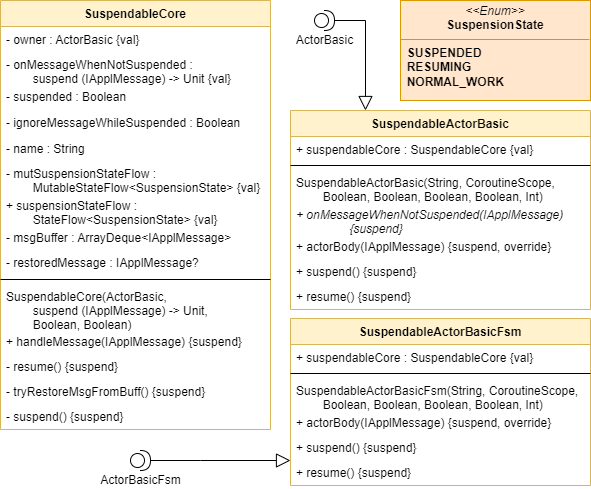
\includegraphics[width=\textwidth]{img/[UML]Suspendable}
	\caption{Suspendable classes}
	\label{fig::suspendable}
\end{figure}

The figure \ref{fig::suspendable} shows the components for the suspension mechanism.
The main classes are \href{https://github.com/LM-96/QA-Extensions/blob/main/it.unibo.qakactor/src/main/kotlin/SuspendableActorBasic.kt}{\texttt{SuspendableActorBasic}} and \href{https://github.com/LM-96/QA-Extensions/blob/main/it.unibo.qakactor/src/main/kotlin/SuspendableActorBasicFsm.kt}{\texttt{SuspendableActorBasicFsm}} and their names suggest their use.

Please notice the class \href{https://github.com/LM-96/QA-Extensions/blob/main/it.unibo.qakactor/src/main/kotlin/SuspendableCore.kt}{\texttt{SuspendableCore}} that is developed in order to make the code very reusable and to limit code repetitions. In addition to all of these classes we also provide \href{https://github.com/LM-96/QA-Extensions/blob/main/it.unibo.qakactor/src/main/kotlin/demo/EchoSuspendableActor.kt}{\texttt{EchoSuspendableActor}} that show some examples of this pausing mechanism.

Without going deeply into details, we can say that this mechanism is based on the \texttt{actorBody} function of the \texttt{ActorBasic} class that is extended by \texttt{SuspendableActorBasic} and \texttt{SuspendableActorBasicFsm}. As you can see in the source code, the overriding methods call the function \texttt{handleMessage} defined into \texttt{SuspendableCore} that is able to decide to handle the message if not pausing or to do something else if the actor is in pause mode. Then, the \texttt{handleMessage} is a sort of \textit{filter} that decides if the message has to be handled.

So, in order to define actors with the ability to go into suspension, the application designer must extend \texttt{SuspendableActorBasic} implementing \texttt{onMessageWhenNotSuspended} or \texttt{SuspendableActorBasicFsm} with the normal procedure used also for \texttt{ActorBasicFsm}. All the job is done by the already implemented \texttt{actorBody} function.

In order to decide if the messages have to be saved into a buffer and restored when resumed or to be discarded, the developer can pass a proper boolean inside the constructor of the suspendable actor classes.
If the messages are stored into a buffer, when the actor receives the \texttt{resume} command, then all the saved messages are restored \textbf{in order} and the actor pass into a \textit{meta-state} that is called \texttt{RESUMING} (see the \texttt{\href{https://github.com/LM-96/QA-Extensions/blob/main/it.unibo.qakactor/src/main/kotlin/SuspendableCore.kt}{\texttt{SuspensionState}}} enumeration). After all messages have been restored, the actor returns at the normal work in the state it was before the suspension.

Notice that as anticipated, we have added a new \textit{layer of state} to the actors that concerns only the \textit{suspension state of the actor} and that is defined by the \texttt{SuspensionState} enumeration.
This kind of state of a \texttt{SuspendableActorBasic} (or \texttt{SuspendableActorBasicFsm}) is observable thanks to the new \href{https://kotlin.github.io/kotlinx.coroutines/kotlinx-coroutines-core/kotlinx.coroutines.flow/-state-flow/}{Kotlin StateFlow} that can be obtained from the owned \texttt{SuspendableCore} of these actors.

\textcolor{ForestGreen}{\textbf{If a suspendable actor is resuming, then also the messages that arrives in this state are enqueued into the buffer. In addition to this, please notice that a finite state machine actor does not really change his \textit{fsm} state during the pause, but it is not able to have the normal work because it is locked by the \texttt{SuspendableCore}.}}

In future development, it is easy to add a new annotation like \texttt{@Suspendable} that marks an actor that can be suspended. It is only required to add the proper support for this kind of annotation to the \texttt{AnnotationLoader} that can inject a \texttt{SuspendableActorBasic}(\texttt{Fsm}) to a \texttt{QActorBasic} instance.